%%%%%%%%%%%%%%%%%%%%%%%%%%%%%%%%%%%%%%%%%
% Simple Sectioned Essay Template
% LaTeX Template
%
% This template has been downloaded from:
% http://www.latextemplates.com
%
% Note:
% The \lipsum[#] commands throughout this template generate dummy text
% to fill the template out. These commands should all be removed when 
% writing essay content.
%
%%%%%%%%%%%%%%%%%%%%%%%%%%%%%%%%%%%%%%%%%

%----------------------------------------------------------------------------------------
%	PACKAGES AND OTHER DOCUMENT CONFIGURATIONS
%----------------------------------------------------------------------------------------
\documentclass[12pt]{article} % Default font size is 12pt, it can be changed here

\usepackage{geometry} % Required to change the page size to A4
\geometry{a4paper} % Set the page size to be A4 as opposed to the default US Letter

\usepackage{graphicx} % Required for including pictures

\usepackage{float} % Allows putting an [H] in \begin{figure} to specify the exact location of the figure

\usepackage{amsmath}
\usepackage{amssymb}

\usepackage{graphicx}
\usepackage{subcaption}

\usepackage{float}
\restylefloat{table}

\usepackage{tabu}

\linespread{1.2} % Line spacing

%\setlength\parindent{0pt} % Uncomment to remove all indentation from paragraphs

\graphicspath{{Pictures/}} % Specifies the directory where pictures are stored

\usepackage[
    backend=biber,
    style=ieee
]{biblatex}
\addbibresource{bibliography.bib}

\usepackage[]{hyperref}
\usepackage{cleveref}


\begin{document}

%----------------------------------------------------------------------------------------
%	TITLE PAGE
%----------------------------------------------------------------------------------------

\begin{titlepage}

\newcommand{\HRule}{\rule{\linewidth}{0.5mm}} % Defines a new command for the horizontal lines, change thickness here

\center % Center everything on the page

\textsc{\LARGE University of York}\\[1.5cm] % Name of your university/college
\textsc{\Large EMBS}\\[0.5cm] % Major heading such as course name
\textsc{\large Embedded Systems Design and Implementation}\\[0.5cm] % Minor heading such as course title

\HRule \\[0.4cm]
{ \huge \bfseries Open Examination 2}\\[0.4cm] % Title of your document
\HRule \\[1.5cm]

\begin{minipage}{0.4\textwidth}
\begin{flushleft} \large
\center \emph{Examination number:}\\
\center Y3606797
\end{flushleft}
\end{minipage}

%\includegraphics{Logo}\\[1cm] % Include a department/university logo - this will require the graphicx package

\vfill % Fill the rest of the page with whitespace

\end{titlepage}

%----------------------------------------------------------------------------------------
%	TABLE OF CONTENTS
%----------------------------------------------------------------------------------------

\tableofcontents % Include a table of contents

\newpage % Begins the essay on a new page instead of on the same page as the table of contents 

%----------------------------------------------------------------------------------------
%	INTRODUCTION
%----------------------------------------------------------------------------------------

\section{Design} % Major section

%------------------------------------------------

The main feature of my design is to split the loops responsible for updating the particles into a piece of hardware using HLS. This loop is the main computation for the simulation and thus it makes sense to optimise it's calculation through custom hardware. Which is what I intended to do with my design iterations. I introduced pipe-lining directives to the inner loop in order to cut the number of clock cycles needed to perform the particle updates. I implemented the pipelined structure within HLS and the result was to cut the maximum latency by a factor of 16, as seen in \cref{Figure:default} and \cref{Figure:pipe-lining}.
	
This design was exported to Vivado and used within the SDK but unfortunately I was unable to get the desired performance from the custom IP, software was outperforming it. Therefore I stuck with the software calculations for the particle updating as I could not put together a working hardware accelerator that actually made a difference in time.

Another loop to optimise within the simulation would be the particle collisions with walls, which I haven't implemented. Again I would attempt to extract some parallelism from the loop by pipe-lining or unrolling.
	
Other design decisions intended to increase performance include: using a fast approximation of the square root function, optimising the length of my loops and other small optimisations.
	
\begin{figure}[h!]
  \centering
  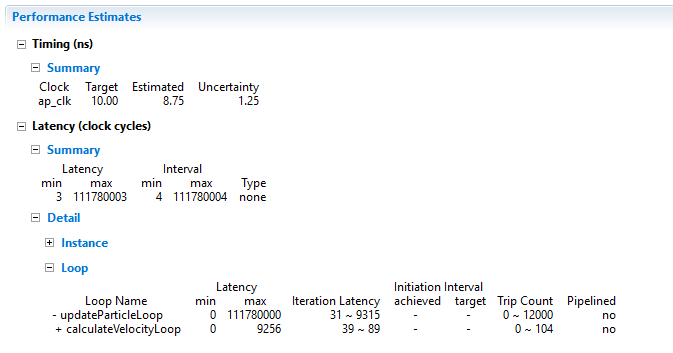
\includegraphics[width=\linewidth]{figures/default.jpg}
  \caption{Before adding any directives}
  \label{Figure:default}
\end{figure}
	
\begin{figure}[h!]
  \centering
  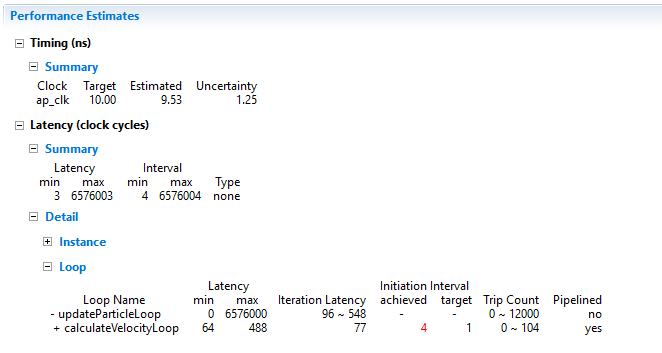
\includegraphics[width=\linewidth]{figures/pipe-lining.jpg}
  \caption{Examples of parallelism within HLS component}
  \label{Figure:pipe-lining}
\end{figure}

\clearpage

\section{Parallelism}

The design makes use of parallelism through the use of pipeline directives in the HLS component. A pipeline allows for parallel execution of what would be otherwise sequential operations in some cases. This can be seen in \cref{Figure:parallel}, the blocks in the same column are operations which are happening in parallel. My two main loops in the particle simulation code do not execute in parallel because their loops do not overlap. Parallelism is still exploited within the loops, but the two loops have a dependence which limits the extent of their parallelism.

Further from this, if we have enough space on the hardware, we could introduce multiple IP blocks to perform a function on different parts of the data in parallel. I explored this option by making two blocks and splitting the memory between them but I couldn't get a working implementation in time.

\begin{figure}[h!]
  \centering
  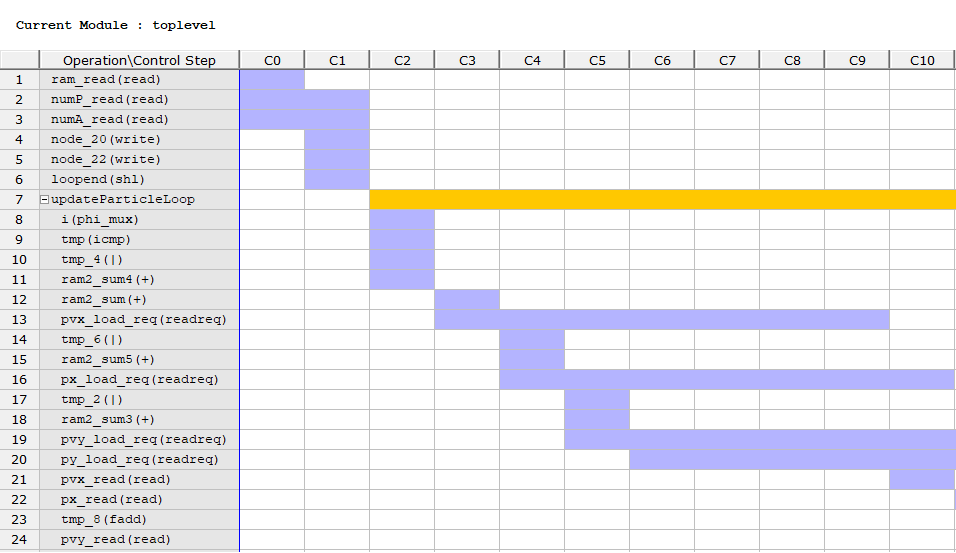
\includegraphics[width=\linewidth]{figures/parallel.jpg}
  \caption{After synthesis with pipeline directives}
  \label{Figure:parallel}
\end{figure}

\section{Testing}

As far as testing the hardware goes, I implemented a simple testbench to verify that my code was performing as expected. In the test bench I populate dummy arrays with dummy data to feed into the toplevel function, then I check that the results are as expected. That formed the majority of the testing with regards to the hardware elements of my system, it is important to test the functionality of your toplevel function because the synthesis of the hardware takes a long time.

To test the rest of the system, I implemented various short-cut keys which can be sent through the serial port to the processor. These short cuts perform the various functions of the particle accelerator \cref{Table:short-cuts}.

\begin{figure}[h!]
\begin{center}
\begin{tabular}{ |c|c| } 
 \hline
Char input & Program function \\
 \hline\hline
 e & Start Ethernet prompt \\ 
 \hline
 r & Start random scenario prompt \\ 
 \hline
 f & Toggle FPS output to uart \\ 
 \hline
\end{tabular}
\end{center}
	\caption{Short-cut keys and functions}
  \label{Table:short-cuts}
\end{figure}

\section{Evaluation}

The design decisions discussed and attempted in my implementation are focused on pure performance enhancements to the particle system, disregarding the usage of memory or hardware on the board in favour of performance.

The utilisation of the board is shown in \cref{Figure:utilisation}, this is the utilisation for the above pipelined examples \cref{Figure:pipe-lining}. My data array was too big to be stored directly in BRAM so I was directly accessing the memory via the port, which results in slower performance overall. To avoid this I could feed in blocks of data at a time to process and return, but I didn't have the time to attempt this for the assessment.

The LUT utilisation was low enough that I had a lot more room for moving functionality from software to hardware, such as wall collisions or perhaps drawing to the frame buffer for the VGA output. Or I could explore using multiple blocks of IP to extract more parallelism from my hardware. 

\begin{figure}[h!]
  \centering
  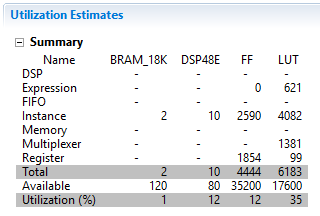
\includegraphics[width=\linewidth]{figures/utilisation.jpg}
  \caption{Board resource utilisation}
  \label{Figure:utilisation}
\end{figure}

\printbibliography 
\end{document}